%!TEX root=paper.tex

\newpage
\section{The System}

The system we present here is that of an open ecosystem: an API at the center allows for varisou implementations of the different components \cite{Lungu16}. However, in order to bootstrap and show its usefulness, we present here our own implementation of several of the components: 

\begin{itemize}
  \item A feed subscription mechanism
  \item An article recommender that craws the selected feeds
  \item An article reader which provides-in place translations
  \item An exercise platform 
\end{itemize}

In the remainder of this section we describe the 


\subsection {Feed Subscription}

When the user indicates that he would like to subscribe to a new source, as explained above, the subscription dialog is displayed. Zeeguu categorizes feeds by their language, and thus we allow users to select any language available and retrieve a list of that language’s sources. Languages are represented by flags, as their compact and iconic representation should be universally understood.

\begin{figure}[h!]
\centering
  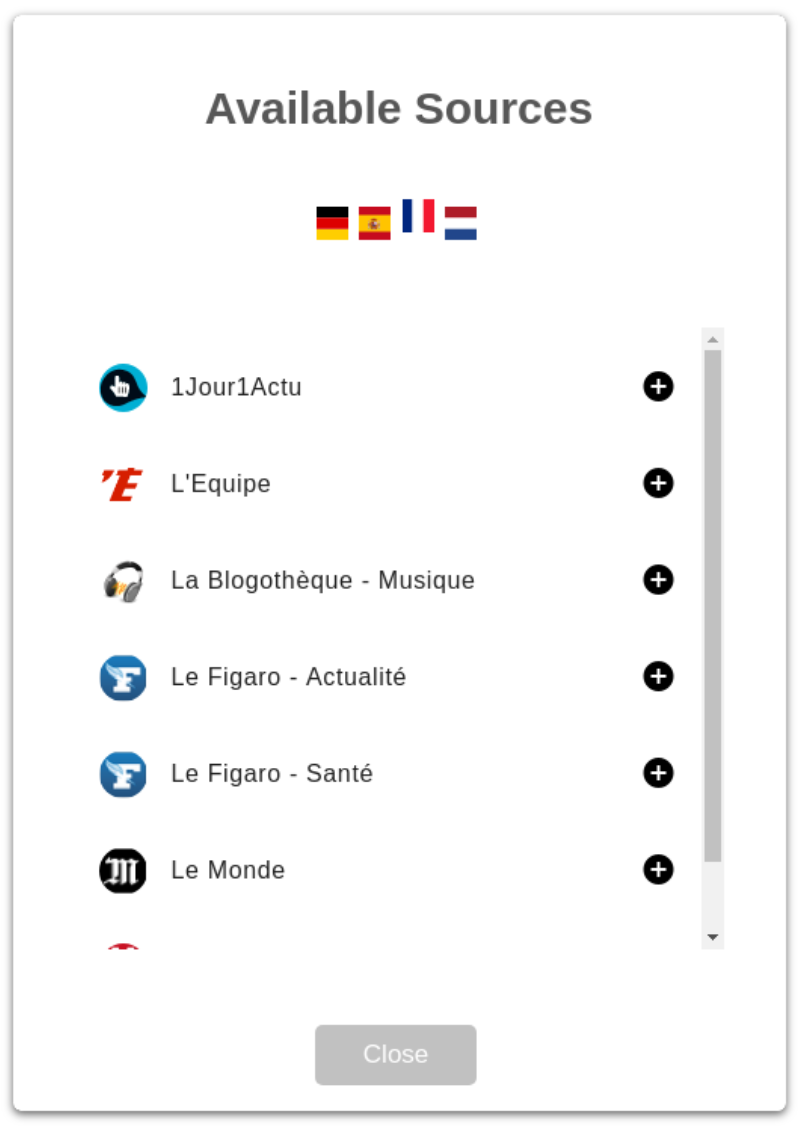
\includegraphics[width=0.5\columnwidth]{figures/available_sources}
  \caption{Different users subscribe to different sources}~\label{fig:registrations}
\end{figure}


\newpage
\subsection{Article Browser}

Article listing presents the source, a summary of the article, and an estimated difficulty level of the article.

In order to properly visualize the reading difficulty of an article in an intuitive manner, there are two levels of information displayed here. First we allow the user to rapidly judge difficulty on an intuitive level by color coding the difficulty from green to yellow to red. When a particular article has grasped the user’s attention, we allow for a more cognitive judgment by scoring the article from 1 to 10 in difficulty.

\begin{figure}[h!]
\centering
  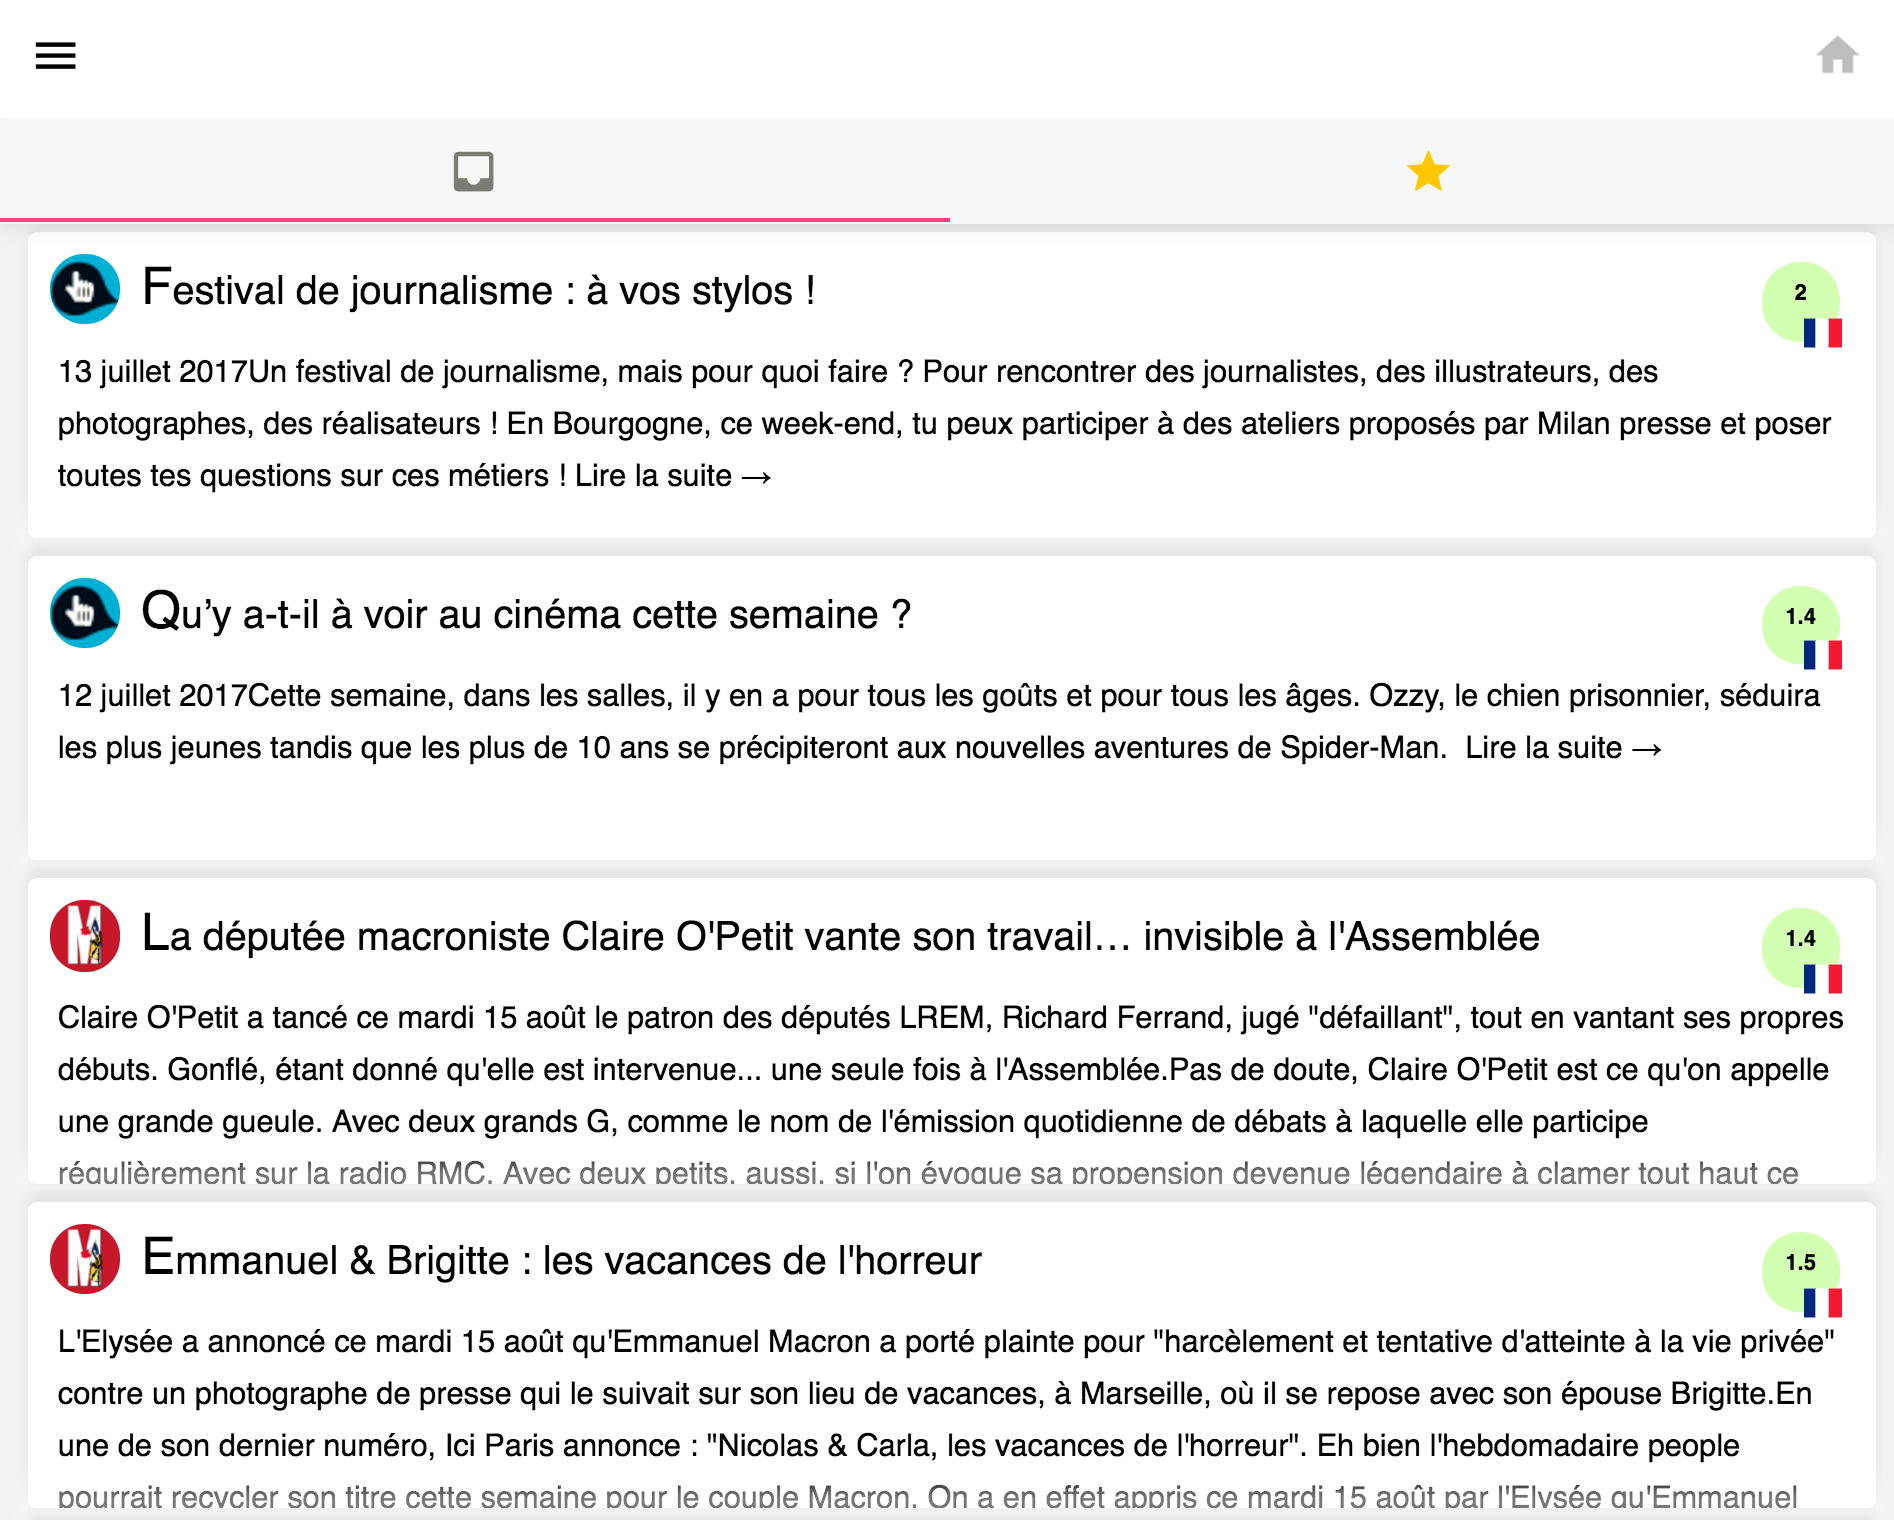
\includegraphics[width=0.7\columnwidth]{figures/article_listing}
  \caption{Article listing presents the source, a summary of the article, and an estimated difficulty level of the article }~\label{fig:registrations}
\end{figure}


\subsection{Article Reader}

The goal of the reader is to make reading as facile as possible. To do this we optimized for the most frequent action that a reader might want to perform. Translating a word. 

We explored several types of interactions and we settled on the following. 
A user clicks on a word, a translation is inserted right after the word. As in the figure: 

\begin{figure}[h!]
\centering
  
\includegraphics[width=0.7\columnwidth]{figures/translated_word}
  \caption{A translated word is inserted after the tapped word.}~\label{fig:registrations}
\end{figure}

\begin{figure}[h!]
\centering
  
\includegraphics[width=0.7\columnwidth]{figures/translated_words1}
  
\includegraphics[width=0.7\columnwidth]{figures/translated_words2}
  \caption{If adjacent words are tapped, this extends the ``translation bubble'' accordingly}~\label{fig:registrations}
\end{figure}

The user can chain a few consecutive words into a single translation if it’s either a phrase that’s new, or if the initially obtained translation needs more words combined with it, to deliver the correct contextual meaning. Again, everything works by tapping the words, as consecutive words will be automati- cally merged into a ’translation bubble’, unifying the entire interaction mode to simple taps on the words (Figure 3). Moreover, this minimalistic interaction model serves another purpose - it is easy to use for words and phrases, but it discourages users to translate entire sentences or even paragraphs, following McCarthy’s [1] idea presented before - extensive reading should discourage intensive use of translations.

One of the limitations of this interaction, that we are still trying to improve is the presence of expressions that are composed of words which are not adjacent (e.g. particle verbs in German and Dutch)


\subsubsection{Alternate Translations}
Since there might be multiple translations possible in a context, one must provide alternatives. Zeeguu does this. We provide exact numbers in a later section, but it can be already specified here that users seem to need to select an alternative about one in eight words.

\begin{figure}[h!]
\centering
  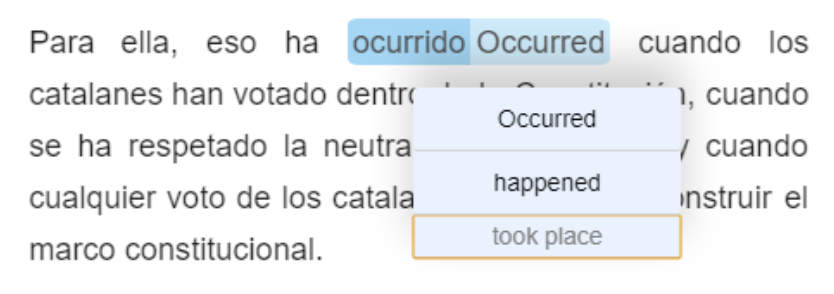
\includegraphics[width=0.8\columnwidth]{figures/translation_alter_menu}
  \caption{A translated word is inserted after the tapped word.}~\label{fig:registrations}
\end{figure}

Moreover, when none of the automatically proposed alternatives is appropriate, the user can upload their own translation.


\subsubsection{Pronounciation}
One of the important features, which was suggested by one of the early expert beta-testers was pronounciation of the given word. Currently this is implemented as a tap on the translated word.


\subsection {Translation Service}

The translations are provided by our server. Besides offering a translation to the reader, the translation service records the word that was translated and its context. This can be used later for two reasons: 

\begin{itemize}
	\item Estimating the current vocabulary of the user
	\item Providing exercises to the reader based on their past reading
\end{itemize}

The translation tries to take context into account when possible. 


This is important since we track the words that the user 


However, even with the multiple possible translations, someties 


\subsection {Exercises}

Given the list of words that a user does not know we can generate exercises for them based on their past readings.

The various interactive elements (IEs) that are present in this exercise (and in some of the other exericses are): 

\begin{itemize}
	\item [IE1] A hint button --
	\item [IE2] Check the answer -- 
	\item [IE3] Word pronunciation -- 
	\item [IE4] Control over the exercise card: report or delete the exercise -- 
	\item [IE5] Input box -- 
\end{itemize}

\begin{figure}[h!]
\centering
  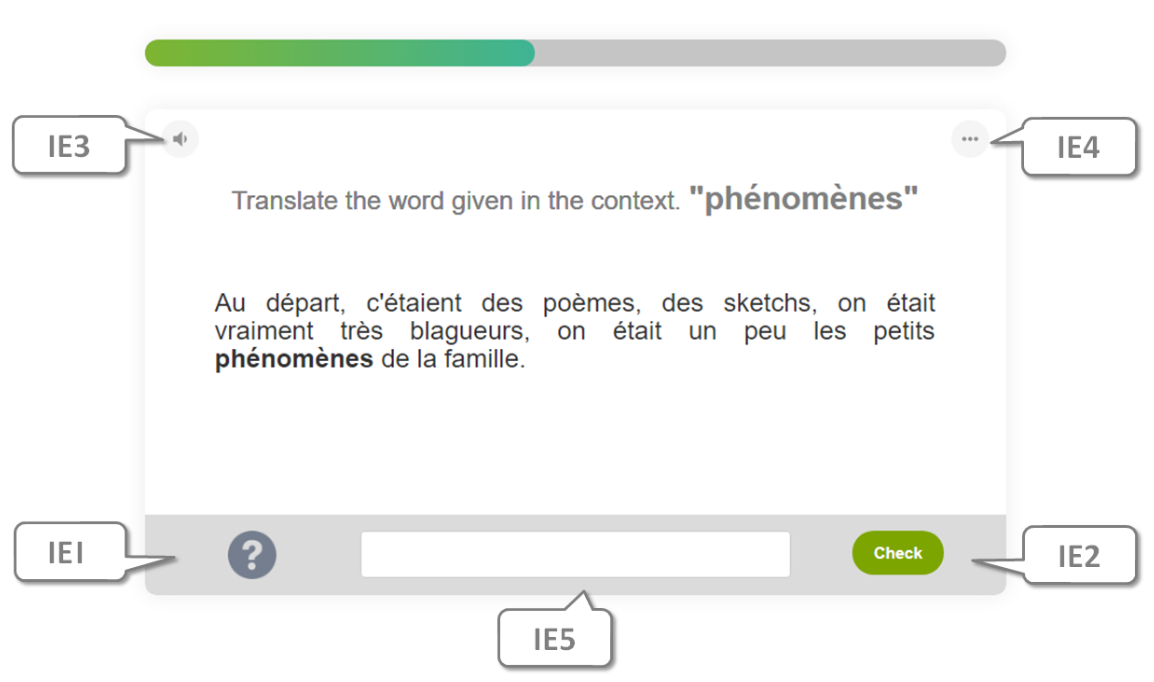
\includegraphics[width=\columnwidth]{figures/exercise_translate}
  \caption{One of the exercise types with which the user is presented. Multiple exercise types are taken from the users past reading context}
\end{figure}



\subsubsection{Scheduling Exercises}

The scheduling algorithm is based on an adaptive, response-time-based scheduling algorithm was developed to increase the efficiency of perceptual learning by Mettler et al. \cite{Mettler14-ARTS}. After evaluating several alternative scheduling strategies we settled on the Mettler one since it has been proven to have gains with both familiar, seen items as well as with new, unseen instances and the benefits of adaptive scheduling were present at an immediate test as well as at a delay \cite{Mettler14-ARTS}.



One of the problems with this is that sometimes the context is too long and sometimes 

